%ARCHITETTURA PLUG-IN
\section{Architettura del prodotto}
Il nostro prodotto\glosp è composto da un plug-in sviluppato per la piattaforma Grafana\glosp e un'applicazione ausiliaria, esterna a tale piattaforma. Perciò l'analisi dell'architettura è suddivisa in queste due componenti.
\subsection{Plug-in}
Per poter visualizzare la suddivisione delle componenti del plug-in e le dipendenze che sussistono tra loro ad alto livello, viene riportato il diagramma dei Package in allegato nel file \textit{diagramma-package-plug-in.png}.
\subsubsection{Progettazione architetturale}
Abbiamo deciso di utilizzare un design pattern architetturale Model-View-Controller (MVC) perché si adatta bene allo sviluppo software all'interno di Grafana\glo. In particolare, come si può vedere nella figura seguente, abbiamo la View che scambia informazioni sulle interazioni dell'utente con il Controller che a sua volta le trasforma in azioni sui dati eseguite da Model. Infine vi è una comunicazione tra Model e View per il costante aggiornamento di quest'ultima, grazie ad una funzionalità fornita dalla piattaforma Grafana\glo.
\mbox{}
\begin{landscape}
	\begin{figure}
		\begin{figure} [H]
			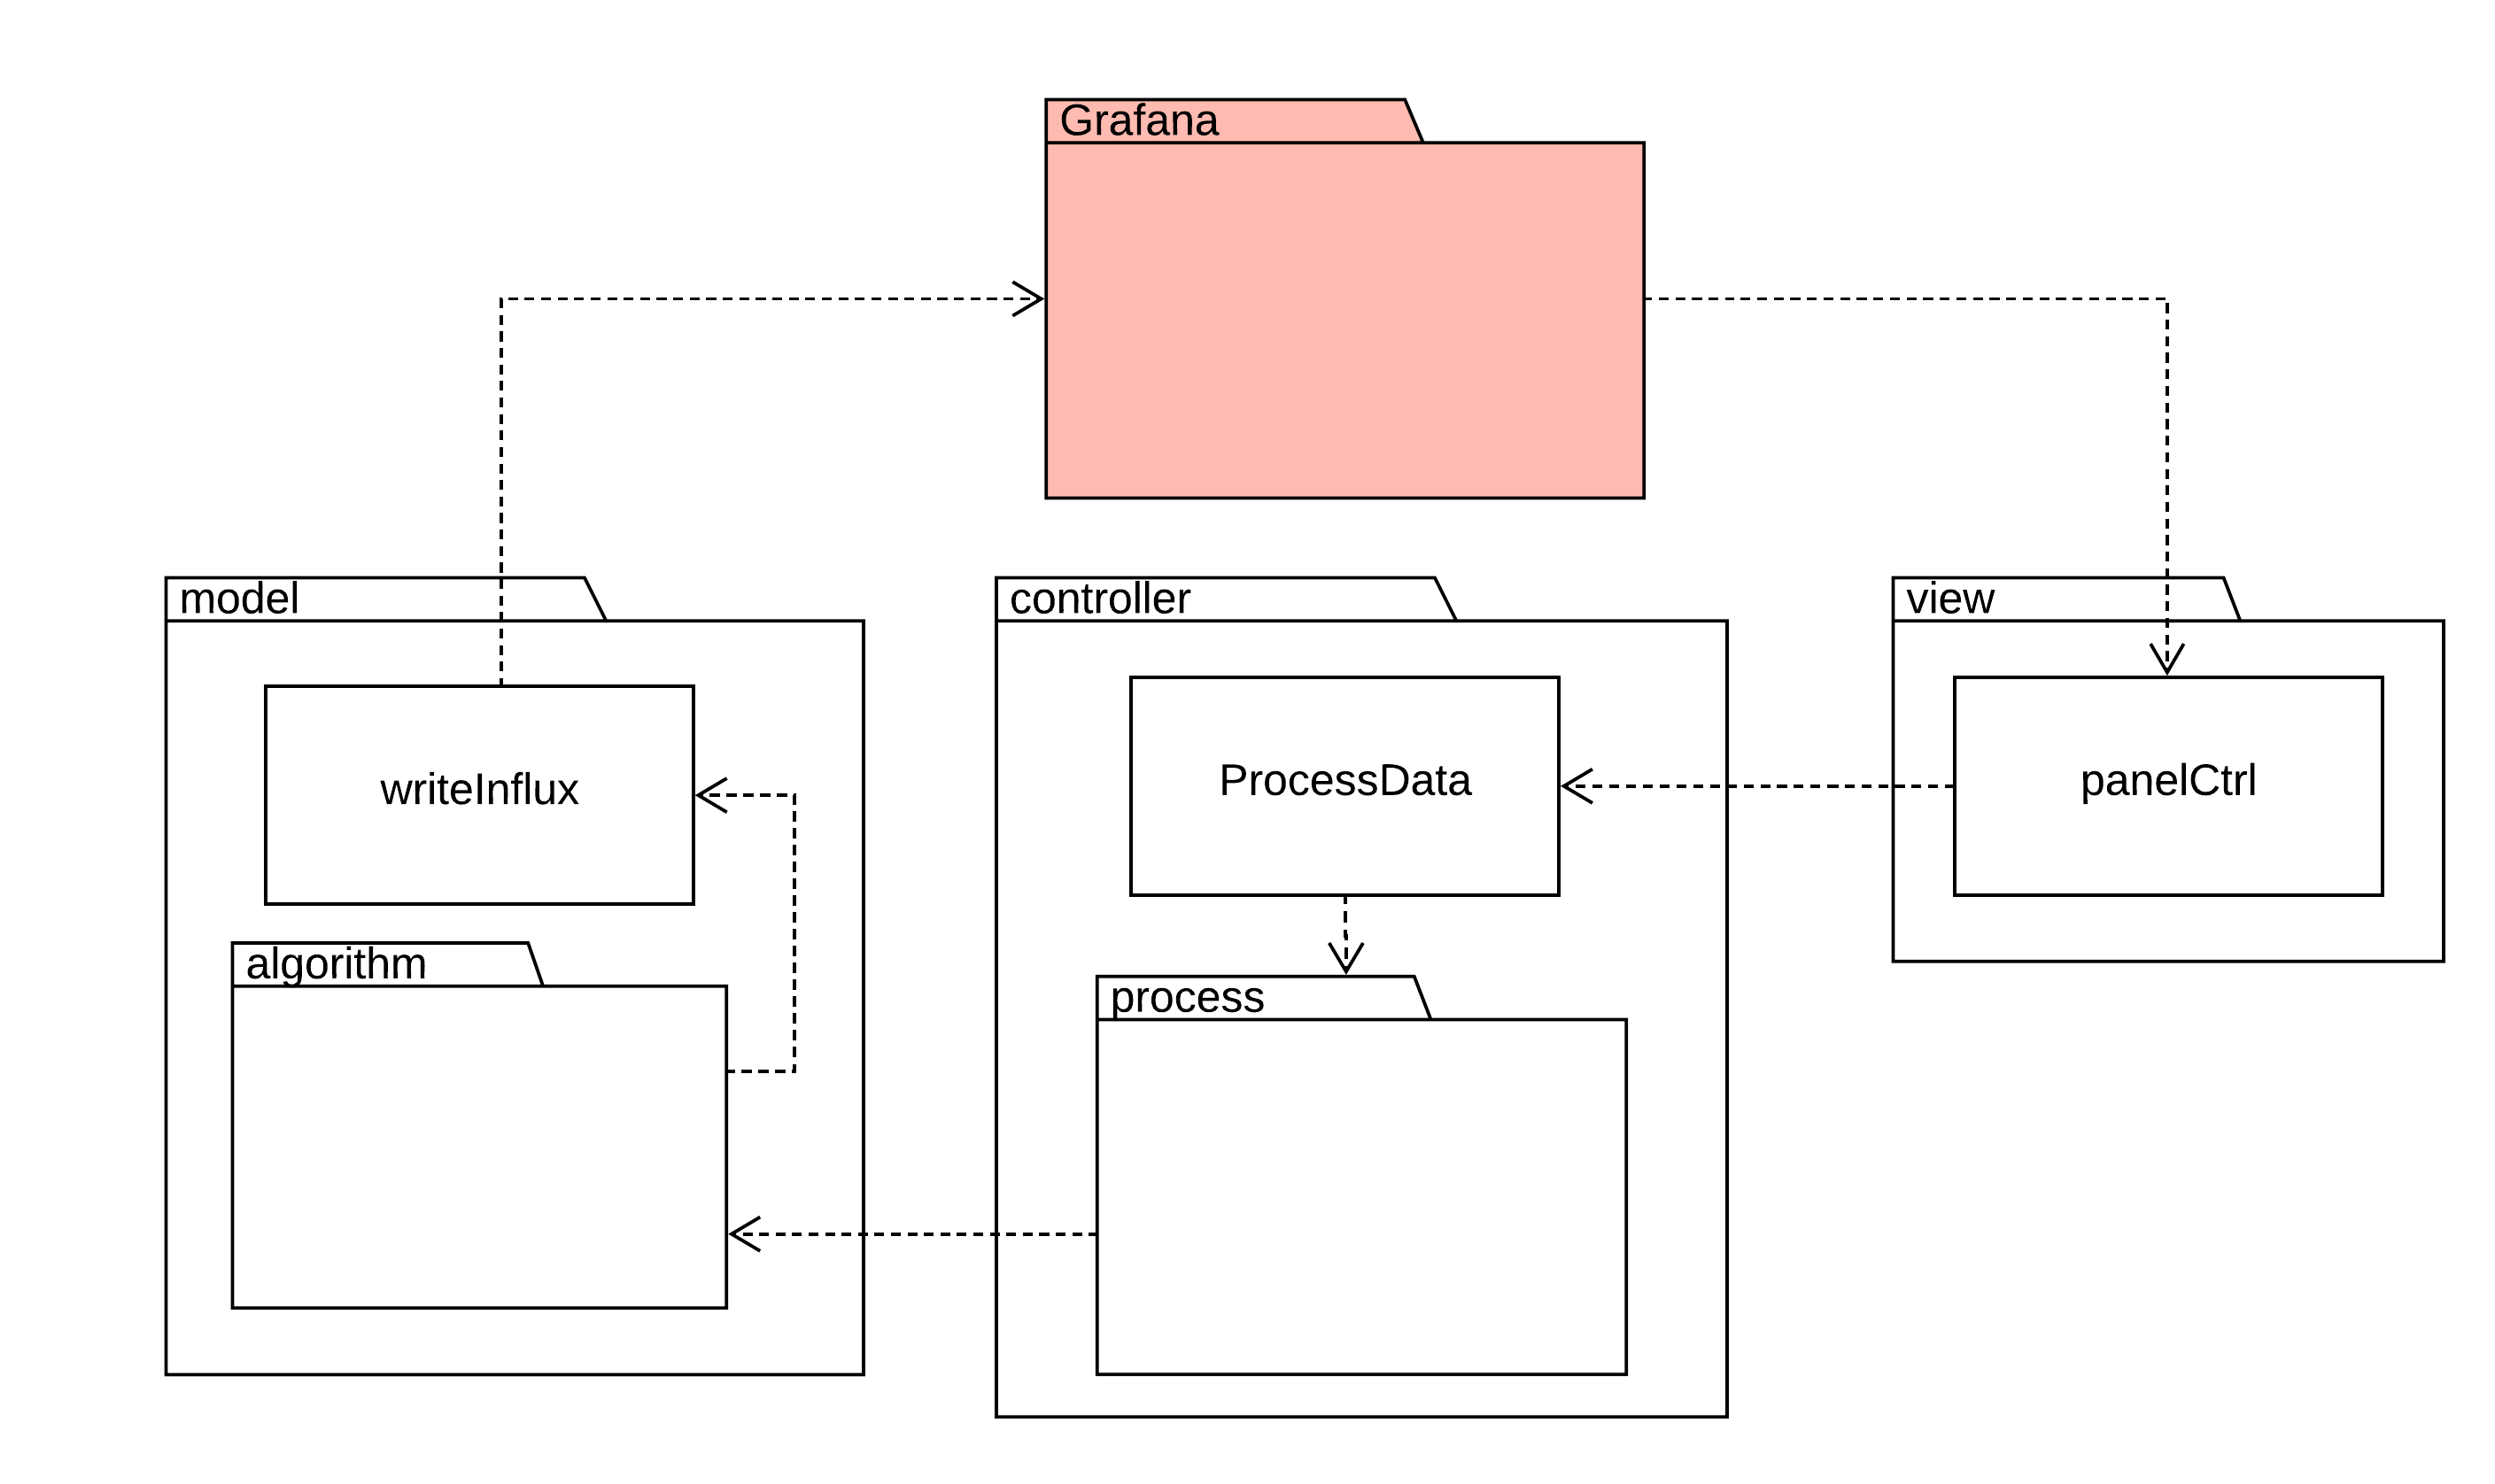
\includegraphics[width=\linewidth]{./img/Diagrammi/architettura-plug-in.png}
			\caption{Diagramma dell'architettura del plug-in}
		\end{figure}
	\end{figure}
\end{landscape}
Analizzando i componenti, la nostra architettura è così strutturata: 
\begin{itemize}
	\item \textbf{Model}: modulo che gestisce la business logic\glo. Più in dettaglio, contiene gli algoritmi di predizione dei dati che sono stati attualmente implementati e la scrittura del risultato delle predizioni su un database Influx;
	\item \textbf{View}: modulo che gestisce la presentation logic. Più in dettaglio, permette la creazione di un pannello grafico personalizzato all'interno di una dashboard Grafana\glo. Con questo pannello l'utente può selezionare le impostazioni degli algoritmi di predizione, i flussi di dati in ingresso, le impostazioni del grafico presente nel pannello e le impostazioni del database influx su cui scrivere i risultati;
	\item \textbf{Controller}: modulo che gestisce l'application logic. Più in dettaglio, trasforma i dati ottenuti dalle interazioni dell'utente ed i flussi dati ottenuti da grafana in un formato adatto per l'esecuzione delle azioni da parte del Model.
\end{itemize}
\subsubsection{Progettazione di dettaglio}
Di seguito viene descritta in dettaglio la progettazione del plug-in. In allegato viene inoltre fornito il file \textit{diagramma-classi-plug-in.png} contenente l'intero diagramma delle classi.
\paragraph{Model} \mbox{}
L'elemento principale contenuto all'interno del modello è il componente degli algoritmi di predizione. Abbiamo implementato due algoritmi di predizione: Support Vector Machine lineare\glosp e Regressione lineare\glo. Esse sono rappresentate rispettivamente dalle classi concrete \textit{SvmPrediction} e \textit{RlPrediction}. In senso più generale abbiamo riscontrato che per le famiglie di algoritmi di Support Vector Machine e di Regressione è possibile ricondursi ad un'interfaccia unica che abbiamo chiamato \textit{AlgorithmPrediction}. Essa fornisce il metodo astratto \textit{predict(data, configuration, influxParameter)} che è implementato dalle classi concrete dei singoli algoritmi.
Queste due classi hanno una dipendenza di tipo composizione con la classe concreta \textit{WriteInflux} che importa la libreria \textit{InfluxDB} e contiene le funzionalità di scrittura su un database Influx. Essa presenta due metodi per la scrittura sul database.
\mbox{}
\begin{landscape}
	\begin{figure}
		\begin{figure} [H]
			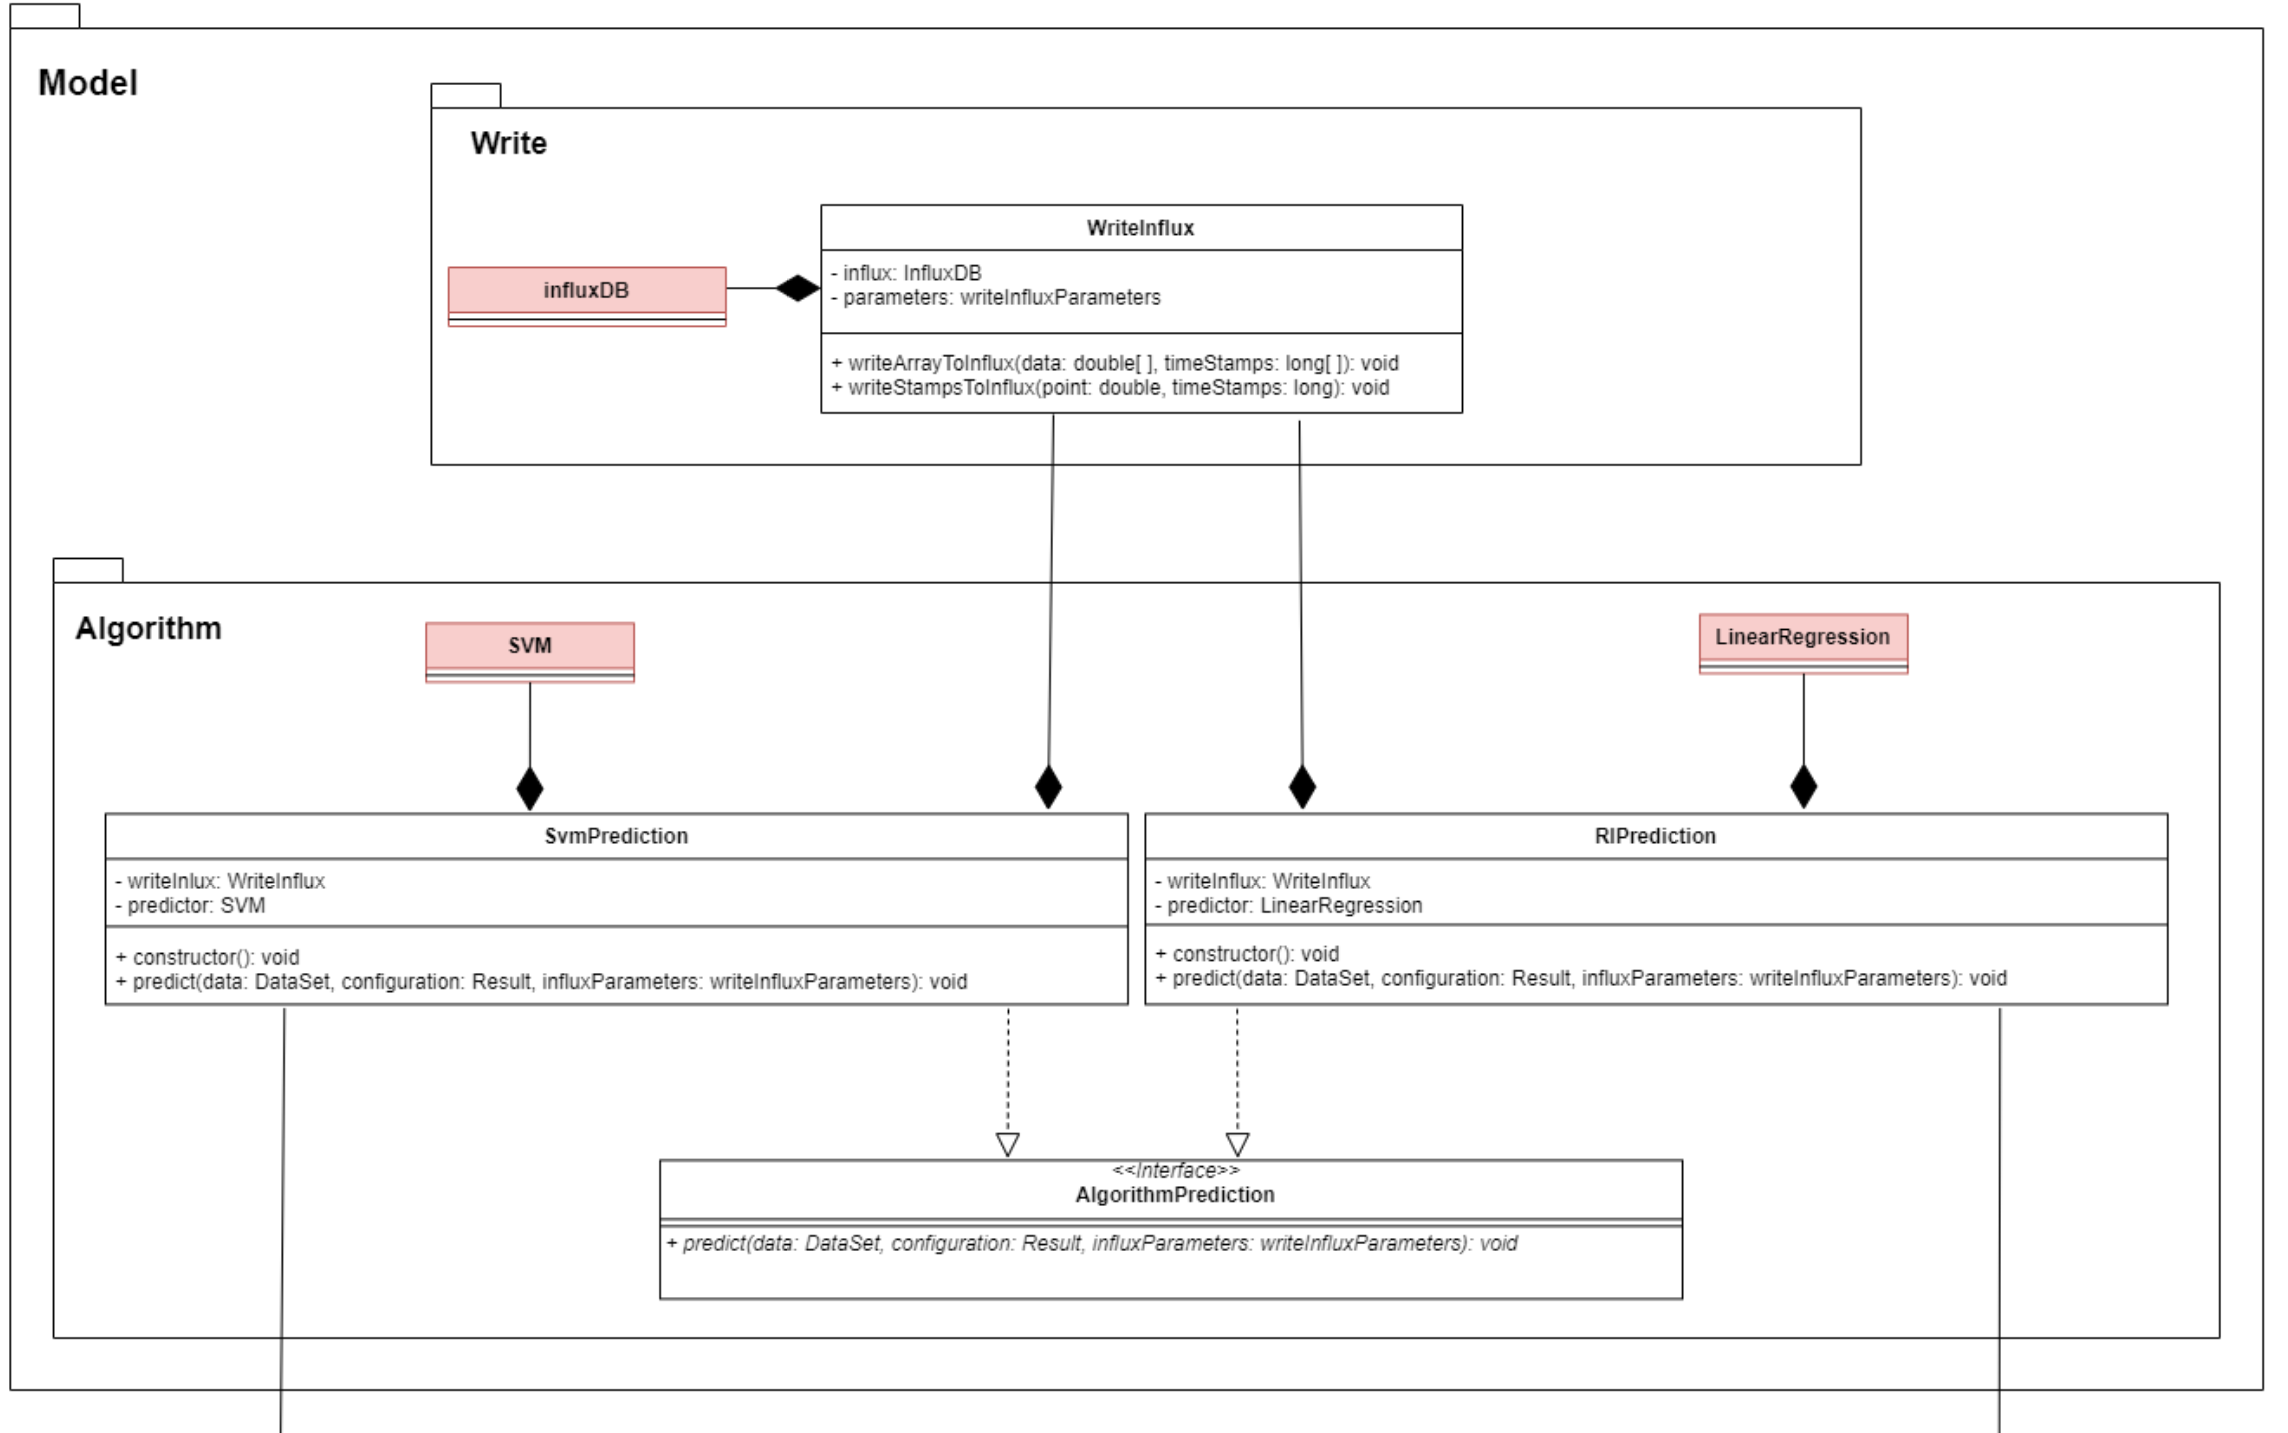
\includegraphics[width=\linewidth]{./img/Diagrammi/model-plug-in.png}
			\caption{Diagramma delle classi del Model}
		\end{figure}
	\end{figure}
\end{landscape}
\paragraph{View} \mbox{}
All'interno della View abbiamo inserito la componente Panel rappresentata dalla classe \textit{PanelCtrl} che estende \textit{MetricPanelControl} di Grafana\glo. Essa rappresenta il nostro pannello principale dal quale gli utenti possono interagire con il plug-in.
Ha una dipendenza di tipo composizione con un componente della libreria Plotly per la creazione del grafico personalizzato e con la classe \textit{SelectinfluxDBCtrl} per la selezione dalla datasource Grafana\glosp di tipo Influx su cui scrivere i risultati delle predizioni. In questo modo, sfruttiamo il meccanismo di Grafana\glosp che dalla scrittura dei dati sul database a questo componente, permette l'aggiornamento continuo della View.
Infine, sempre all'interno di \textit{PanelCtrl}, c'è una dipendenza verso il componente \textit{ProcessData} del Controller che ne permette il collegamento.
\mbox{}
\begin{landscape}
	\begin{figure}
		\begin{figure} [H]
			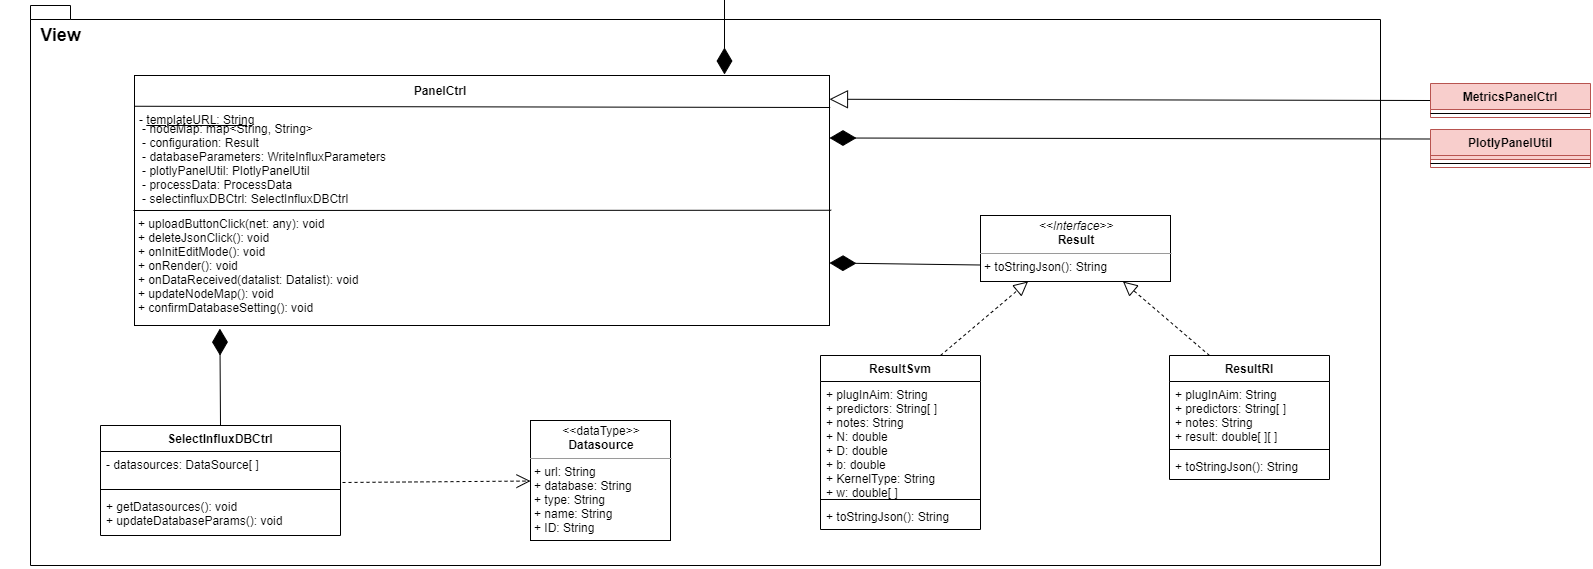
\includegraphics[width=\linewidth]{./img/Diagrammi/view-plug-in.png}
			\caption{Diagramma delle classi della View}
		\end{figure}
	\end{figure}
\end{landscape}
\paragraph{Controller} \mbox{}
All'interno del Controller viene implementata la trasformazione dei dati ricevuti dalla View, che rappresentano le interazioni dell'utente con il nostro pannello ed i flussi di dati ottenuti da Grafana\glo, ad azioni da eseguire sul Model.
Abbiamo deciso di implementare un design pattern strategy ottenendo la seguente struttura:
\begin{itemize}
	\item \textbf{ProcessData}: è una classe concreta che rappresenta il context del nostro strategy. Al suo interno, infatti, viene scelto quale algoritmo di predizione processare sulla base dei dati e delle richieste ricevute. Inoltre essa ha una dipendenza di tipo aggregazione con l'interfaccia \textit{PerformPrediction};
	\item \textbf{PerformPrediction}: è un'interfaccia che rappresenta la strategia astratta. Essa definisce il contratto da rispettare per poter implementare una nuova classe concreta che processa i dati da fornire ad un determinato algoritmo;
	\item \textbf{ProcessSvm}: è una classe concreta che implementa \textit{PerformPrediction} e rappresenta il componente che processa e trasforma i dati da fornire per l'esecuzione dell'algoritmo Svm\glosp sul Model;
	\item \textbf{ProcessSvm}: è una classe concreta che implementa \textit{PerformPrediction} e rappresenta il componente che processa e trasforma i dati da fornire per l'esecuzione dell'algoritmo Rl sul Model.
\end{itemize}
\mbox{}
\begin{landscape}
	\begin{figure}
		\begin{figure} [H]
			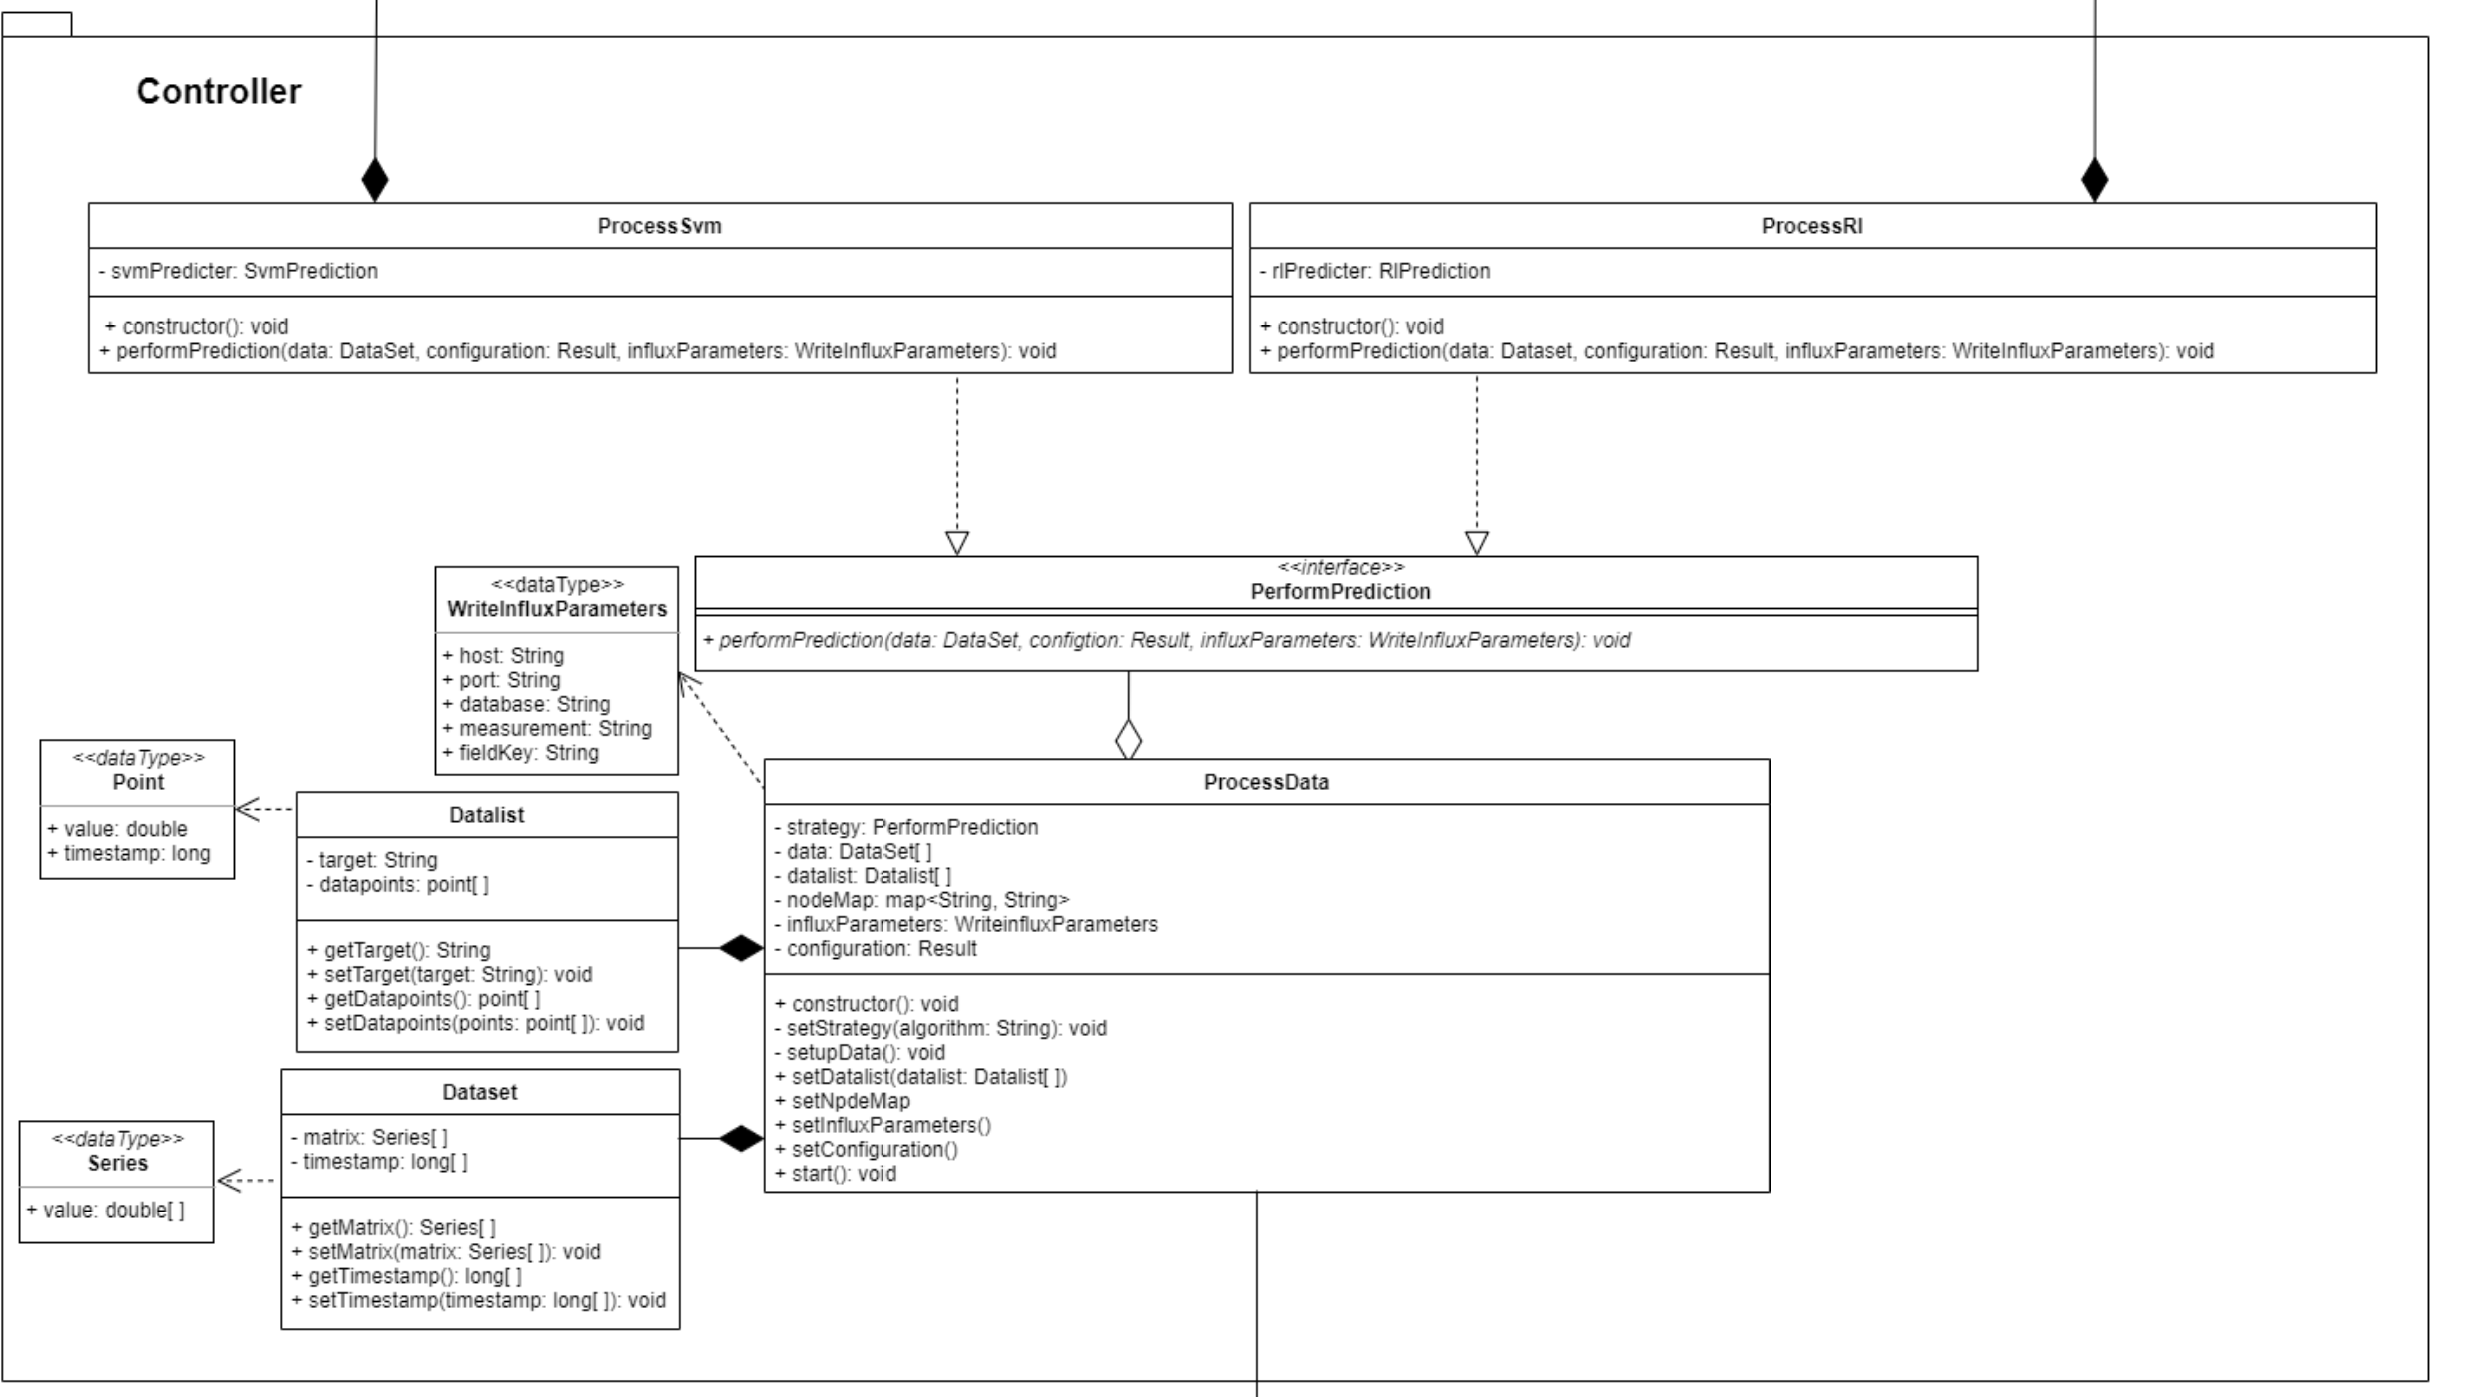
\includegraphics[width=\linewidth]{./img/Diagrammi/controller-plug-in.png}
			\caption{Diagramma delle classi del Controller}
		\end{figure}
	\end{figure}
\end{landscape}
Per spiegare meglio l'insieme di azioni compiute al fine di processare i dati per eseguire la predizione degli algoritmi, illustriamo un diagramma di sequenza che prende in esame SVM\glo. Il procedimento è indicativo anche per gli altri algoritmi.
\mbox{}
\begin{landscape}
	\begin{figure}
		\begin{figure} [H]
			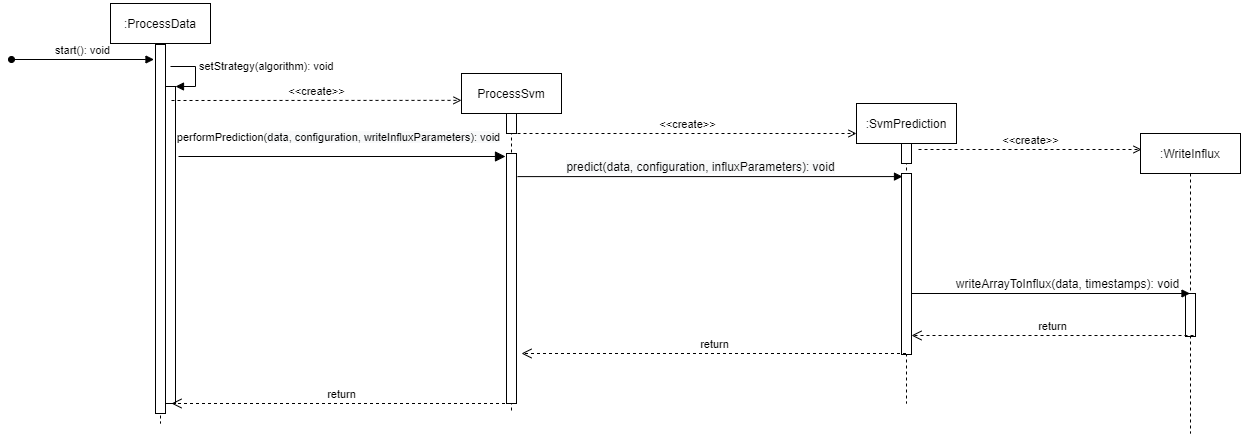
\includegraphics[width=\linewidth]{./img/Diagrammi/ds-plug-in.png}
			\caption{Diagramma di sequenza di processo dei dati per SVM}
		\end{figure}
	\end{figure}
\end{landscape}
